\section{Cubic Spline Interpolation}

\begin{bigidea}
Given $N+1$ points $(t_0,y_0),\dots,(t_N,y_N)$, a cubic spline is a piecewise cubic polynomial defined by a different polynomial $p_k(t)$ for each subinterval $[t_{k-1},t_k]$, $k=1,\dots,N$.
\end{bigidea}

\begin{definition}
Consider $N+1$ points $(t_0,y_0),\dots,(t_N,y_N)$. A {\bf cubic spline} \cite[p.326]{MH} interpolating the data is a function $p(t)$ defined piecewise by $N$ cubic polynomials $p_1(t),\dots,p_N(t)$ where
$$
p_k(t) = a_k(t - t_{k-1})^3 + b_k(t - t_{k-1})^2 + c_k(t - t_{k-1}) + d_k \ \ , \ \ t \in [t_{k-1},t_k]
$$
such that $p(t)$, $p'(t)$ and $p''(t)$ are continuous functions.
\end{definition}

\begin{note}
Each polynomial $p_k(t)$ has 4 coefficients $a_k,b_k,c_k,d_k$ therefore we require $4N$ equations to specify the $4N$ unknowns:
\begin{enumerate}
\item Interpolation at left endpoints: $p_k(t_{k-1}) = y_{k-1}$ for $k=1,\dots,N$ yields $N$ equations.
\item Interpolation at right endpoints: $p_k(t_k) = y_k$ for $k=1,\dots,N$ yields $N$ equations.
\item Continuity of $p'(t)$: $p_k'(t_k) = p_{k+1}'(t_k)$ for $k=1,\dots,N-1$ yields $N-1$ equations.
\item Continuity of $p''(t)$: $p_k''(t_k) = p_{k+1}''(t_k)$ for $k=1,\dots,N-1$ yields $N-1$ equations.
\end{enumerate}
The conditions impose only $4N-2$ equations therefore we need 2 more to determine the cubic spline uniquely. There are different choices such as the natural spline and the ``not-a-knot" condition. See \cite[p.327]{MH}.
\end{note}

\begin{definition}
The {\bf natural cubic spline} \cite[p.327]{MH} requires $p''_1(t_0) = p''_N(t_N) = 0$.
\end{definition}

\begin{definition}
Represent a cubic spline $p(t)$ by the {\bf coefficient matrix}
$$
C=
\begin{bmatrix}
a_1 & a_2 & \cdots & a_N \\
b_1 & b_2 & \cdots & b_N \\
c_1 & c_2 & \cdots & c_N \\
d_1 & d_2 & \cdots & d_N
\end{bmatrix}
$$
where the $k$th column of $C$ consists of the coefficients for the $k$th cubic polynomial in the spline
$$
p_k(t) = a_k(t - t_{k-1})^3 + b_k(t - t_{k-1})^2 + c_k(t - t_{k-1}) + d_k \ \ , \ \ t \in [t_{k-1},t_k]
$$
\end{definition}

\begin{proposition}
Consider $N+1$ points $(t_0,y_0),\dots,(t_N,y_N)$ (with $t_i \not= t_j$ for $i \not= j$). The unique natural cubic spline $p(t)$ which interpolates the points is given by the coefficient matrix
$$
C=
\begin{bmatrix}
a_1 & a_2 & \cdots & a_N \\
b_1 & b_2 & \cdots & b_N \\
c_1 & c_2 & \cdots & c_N \\
d_1 & d_2 & \cdots & d_N
\end{bmatrix}
$$
where $d_k = y_{k-1}$ for $k=1,\dots,N$ and the coefficients $a_1,b_1,c_1,\dots,a_N,b_N,c_N$ are the solution of the linear system
$$
\renewcommand{\arraystretch}{1.5}
\left[ \begin{array}{c|c|c|c|c}
A(L_1) & B & & & \\ \hline
& A(L_2) & B & & \\ \hline
& & \ddots & \ddots & \phantom{A(L_{N-1})} \\ \hline
\phantom{A(L_{N-1})} & \phantom{A(L_{N-1})} & \phantom{A(L_{N-1})} & A(L_{N-1}) & B \\ \hline
T & & & & V
\end{array} \right]
\renewcommand{\arraystretch}{1}
\begin{bmatrix} a_1 \\ b_1 \\ c_1 \\ \vdots \\ a_N \\ b_N \\ c_N \end{bmatrix}
=
\begin{bmatrix} y_1 - y_0 \\ 0 \\ 0 \\ \vdots \\ y_N - y_{N-1} \\ 0 \\ 0 \end{bmatrix}
$$
where $L_k = t_k - t_{k-1}$ is the length of the subinterval $[t_{k-1},t_k]$ and
$$
A(L) = \begin{bmatrix} L^3 & L^2 & L \\ 3L^2 & 2L & 1 \\ 6L & 2 & 0 \end{bmatrix}
\ \
B = \left[ \begin{array}{rrr} 0 & 0 & 0 \\ 0 & 0 & -1 \\ 0 & -2 & 0 \end{array} \right]
\ \
T = \begin{bmatrix} 0 & 0 & 0 \\ 0 & 2 & 0 \\ 0 & 0 & 0 \end{bmatrix}
\ \
V = \begin{bmatrix} L_N^3 & L_N^2 & L_N \\ 0 & 0 & 0 \\ 6L_N & 2 & 0 \end{bmatrix}
$$
\end{proposition}

\begin{example}
Construct the natural cubic spline interpolating points
$$
(0,0),(1,2),(2,1),(3,3),(4,2),(5,4),(6,2),(7,3),(8,1),(9,2),(10,0)
$$
\begin{center}
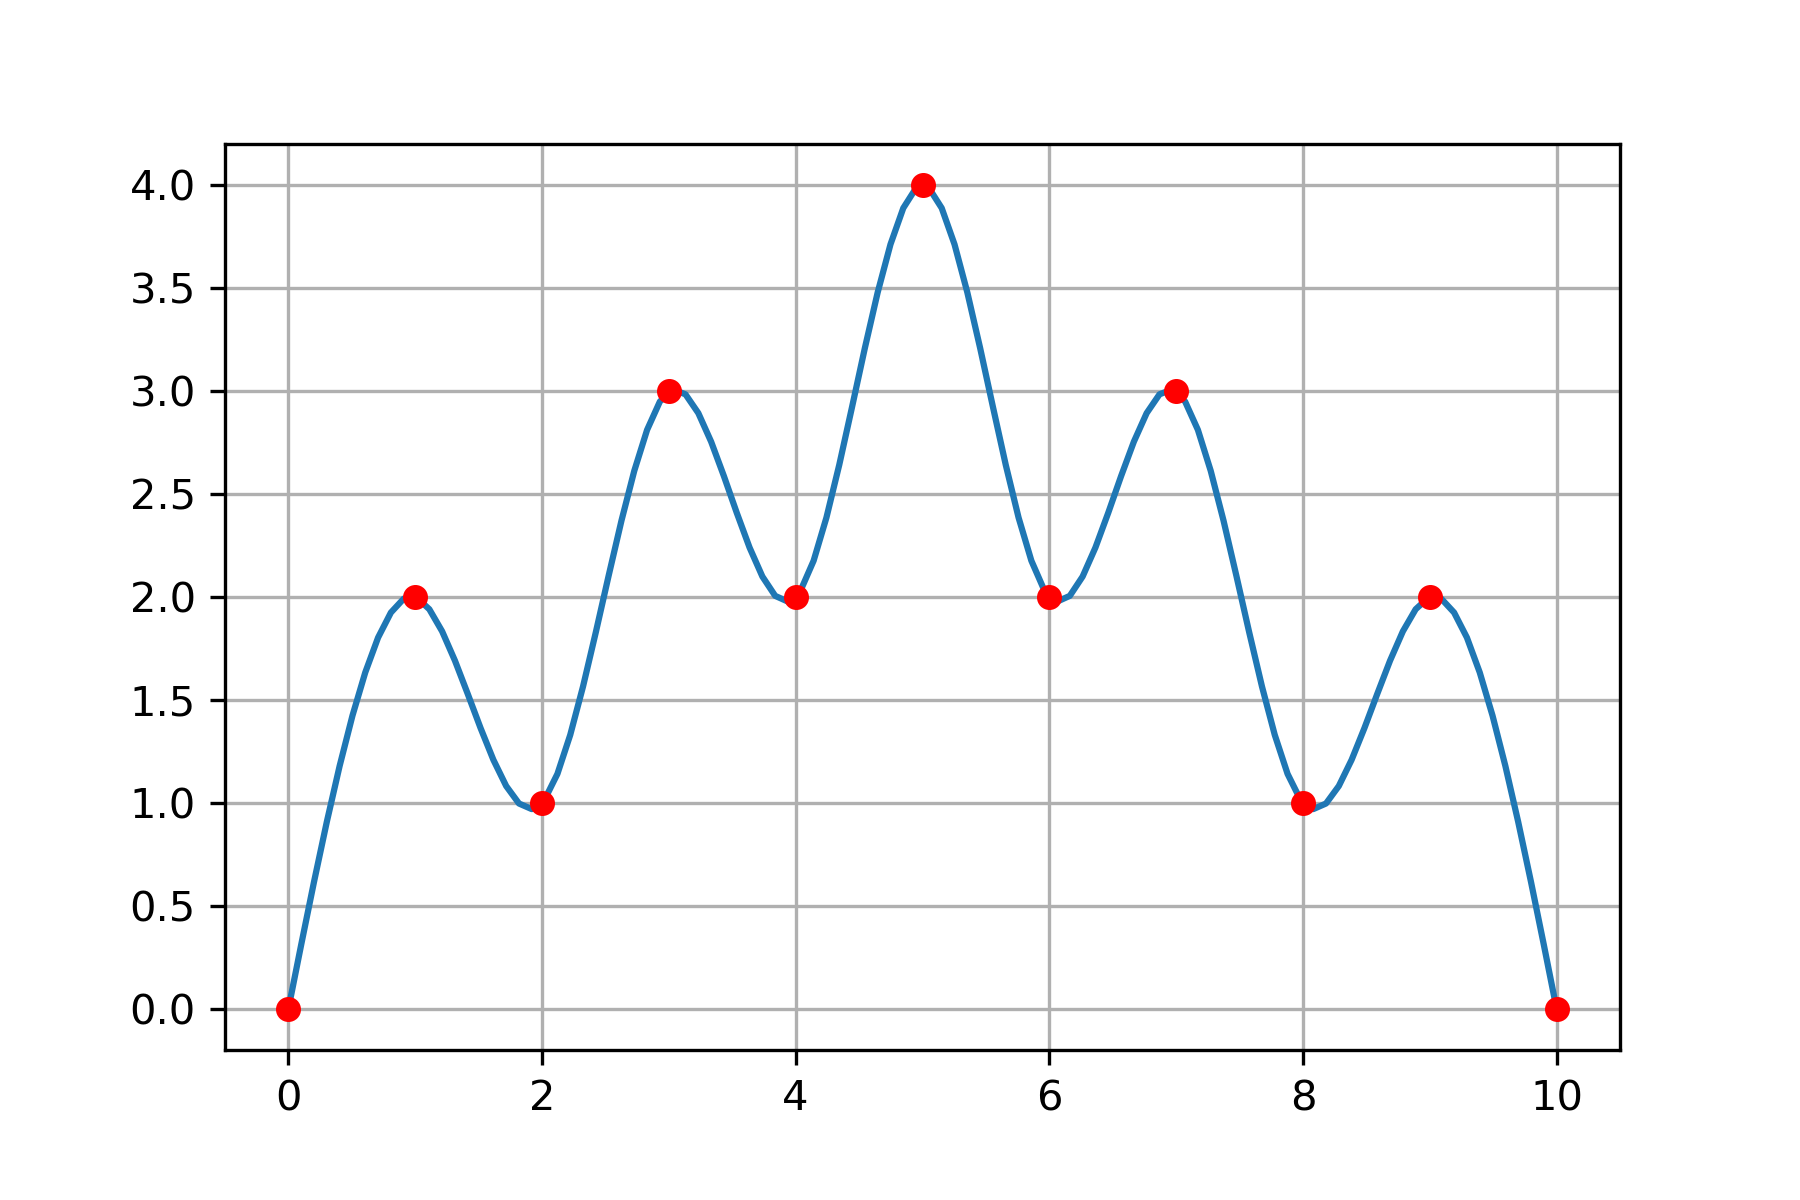
\includegraphics[width=3.5in]{01_06_img01.png}
\end{center}
\end{example}

\begin{note}
The condition number of the matrix for constructing the natural cubic spline does not increase as drastically with the number of points $N+1$ as compared with the Vandrmonde matrix. For example, for $11$ equally spaced points $t_0=0,\dots,t_{10}=10$, the Vandermonde matrix is 11 by 11 and has $\mathrm{cond}(A) \approx 10^{12}$ whereas the cubic spline matrix is 30 by 30 and the condition number is only around $33$.
\begin{center}
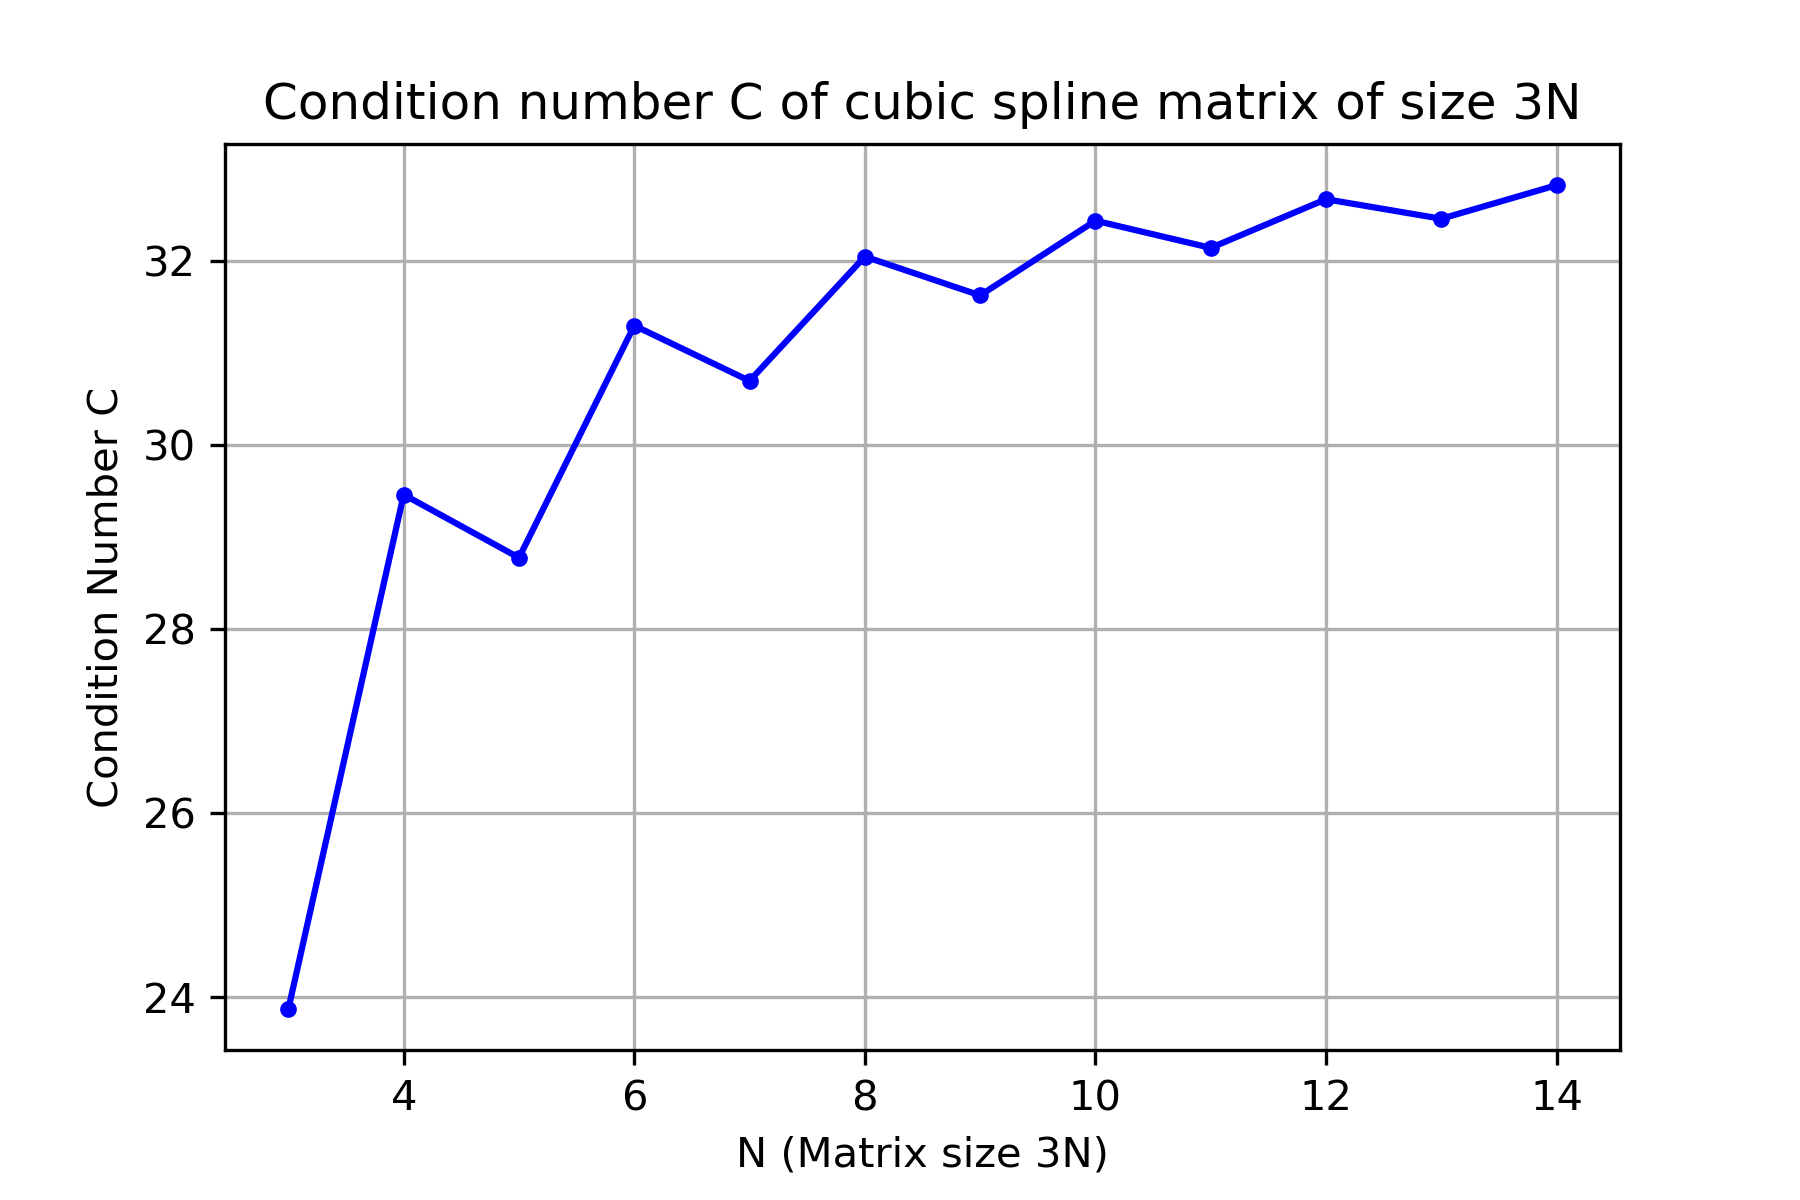
\includegraphics[width=3.5in]{01_06_img02.png}
\end{center}
\end{note}